\chapter{Methodology}
The primary goal of this thesis is to achieve the swing-up movement in the pendubot or acrobot setup and to maintain stability around the highest points. Challenges have been revealed in initial training trials with reinforcement learning, including potential entrapment in local minima and difficulty in maintaining stability at the highest point for extended periods.

To address these challenges, two main strategies are adopted. For the stabilization issue, a combined controller is introduced. During the swing-up process, control is assumed by an RL-trained agent, utilizing the Soft Actor-Critic—a classic model-free reinforcement learning algorithm—based on its learned policies. However, as the system nears the maximum point, a seamless transition occurs. This shift allows for the takeover of control by a continuous-time LQR controller, ensuring the final stabilization required to maintain stability at the highest point. For the entrapment in local minima problem, a carefully designed reward function is utilized to guide the agent away from hazadous local minima and achieve successful swing up.

\section{Soft actor critic}
Within the landscape of reinforcement learning, the Soft Actor Critic (SAC)\cite{haarnoja2018soft} stands out as an algorithm specifically designed for environments with continuous state and action spaces. Such environments, exemplified by our double pendulum system where actuators can be adjusted to any value within the torque limit range, and state measurement can take any real number, influenced our decision to adopt SAC.

Like many other deep reinforcement learning algorithms, SAC optimizes a policy by maximizing the expected cumulative reward the agent obtains over time. This optimization is primarily achieved through an actor-critic structure\cite{konda1999actor}.

The actor determines the best actions by interpreting the current environmental conditions and adhering to the existing policy. Typically, the actor is visualized as a shallow neural network that approximates the mapping between the input state and the output probability distribution over actions. Furthermore, SAC incorporates a stochastic policy within its actor, which fosters exploration and aids the agent in refining its policies.

On the other hand, the critic evaluates the value of state-action pairs. It estimates the expected cumulative reward the agent can achieve by following a particular policy. More often than not, the critic is depicted as a neural network that processes state-action pairs as inputs to yield the estimated value.

A distinguishing feature of SAC, besides the actor-critic framework, is entropy regularization\cite{achiam2018spinning}. SAC utilizes a stochastic policy. This means that instead of always settling on a single best action for each state, the agent considers a probability distribution over potential actions. The incorporation of entropy in SAC aims to encourage exploration: high entropy signifies a more uniform distribution, implying the agent's uncertainty and tendency to explore diverse actions, while low entropy points to a concentrated distribution, suggesting the agent's confidence in a specific action. By definition, entropy quantifies randomness. Within SAC, it captures the unpredictability of the policy's action distribution. If
\(x\) is a random variable with a probability density function \(P\), the
entropy \(H\) of \(x\) is defined as:

\begin{equation}
 H(P) = \displaystyle \mathop{\mathbb{E}}_{x \sim P}[-\log P(x)]
\end{equation}

By maximizing entropy, SAC encourages exploration and accelerates learning. It
also prevents the policy from prematurely converging to a suboptimal solution.
The trade-off between maximizing reward and maximizing entropy is controlled
through a parameter, \(\alpha\). This parameter serves to balance the importance
of exploration and exploitation within the optimization problem. Each interactioin between the agent and the environment can be recorded as a tuple \((s_t,a_t,R,s_{t+1})\). The optimal policy
\(\pi^*\) can be defined as follows:

\begin{equation}
 \pi^* = {arg}{\max_{\pi}}{\displaystyle
 \mathop{\mathbb{E}}_{\tau\sim\pi}}{\Bigg[{\sum_{t=0}^{\infty}}{\gamma^{t}}{\Big(R(s_t,a_t,s_{t+1})}+{\alpha}H(\pi(\cdot\mid{s_t}))\Big)\Bigg]}
\end{equation}

Where \(s_t\) and \(a_t\) represent the state and action at time \(t\), and \(s_{t+1}\) represents the state at time \(t+1\). \(R\) denotes the immediate reward received by the agent after taking action \(a_t\) in state \(s_t\), while \(\gamma\) is the discount factor that determines the agent's emphasis on long-term cumulative rewards over immediate ones.

During training, SAC learns a policy $\pi_{\theta}$ and two Q-functions
$Q_{\phi_1} , Q_{\phi_2}$ concurrently. The loss functions for the two Q-networks are
$(i \in {1, 2})$:

\begin{equation}
  L(\phi_i,D) = \displaystyle
  \mathop{\mathbb{E}}_{(s,a,r,s',d)\sim{D}}\bigg[\bigg(Q_{\phi_i}(s,a)-y(r,s',d)\bigg)^2\bigg],
\end{equation}

where the temporal difference target \(y\) is given by:

\begin{align}
  y(r,s',d) &= r + \gamma(1-d) \times \nonumber\bigg(\displaystyle
  \mathop{\min}_{j=1,2}Q_{\phi_{targ,j}}(s',\tilde{a}')-\alpha\log
  {\pi_\theta}(\tilde{a}'\mid{s}')\bigg), \\
  \tilde{a}'&\sim{\pi_\theta}(\cdot\mid{s'})
\end{align}

In each state, the policy \(\pi_\theta\) should act to maximize the expected
future return \(Q\) while also considering the expected future entropy \(H\). In other
words, it should maximize \(V^\pi(s)\):

\begin{align}
 V^\pi(s) &= {\displaystyle \mathop{\mathbb{E}}_{a\sim\pi}[Q^\pi(s,a)]} +
 \alpha{H(\pi(\cdot\mid{s}))} \\
 &= {\displaystyle \mathop{\mathbb{E}}_{a\sim\pi}[Q^\pi(s,a)} -
 \alpha{\log {\pi(a\mid{s})]}}
\end{align}

The interaction experiences are stored as tuples \((s, a, r, s', d)\) in a replay buffer \(\textit{D}\). Here, \(d\) represents the signal for episode termination. When it is time to update the Q-value and policy, a batch of transitions \(\textit{B} = \{(s, a, r, s', d)\}\) is randomly sampled from \(\textit{D}\). The Q-functions are updated by one step of gradient descent, the gradients of the loss functions for the Q-networks are calculated by:

\begin{equation}
\nabla_{\phi_i} \frac{1}{|\textit{B}|} \sum_{(s, a, r, s', d) \in \textit{B}} \left(Q_{\phi_i}(s, a) - y(r, s', d)\right)^2 \quad \text{for} \quad i=1,2
\end{equation}

The policy is updated using one step of gradient ascent, the gradient is expressed as:

\begin{equation}
\nabla_{\theta} \frac{1}{|\textit{B}|} \sum_{s \in \textit{B}}\left(\min\limits_{\substack{i=1,2}}Q_{\phi_i}(s,\widetilde{a}_{\theta}(s)) - \alpha \log\pi_{\theta}(\widetilde{a}_{\theta}(s)|s)\right)
\end{equation}

where \(\widetilde{a}_{\theta}(s)\) is a sample of action derived from \(\pi_\theta(\cdot|s)\) which is differentiable with respect to \(\theta\). 

In conclusion, SAC's combination of stochastic policies, exploration through
entropy regularization, value estimation, and gradient-based optimization make
it a well-suited algorithm for addressing the challenges posed by continuous
state and action spaces.

\section{Linear quadratic regulator}
The Linear Quadratic Regulator (LQR)\cite{lehtomaki1981robustness} is an effective control method primarily designed for linear systems. Yet, when dealing with nonlinear dynamics, it remains applicable. The nonlinear system is linearized around a selected operating point, and based on this linearized version, the LQR controller can be sculpted.

Taking a step back, the general form of a nonlinear system defined by state vector \(x\) and input vector \(u\) can be expressed as:
\begin{equation}
 \dot{x}(t) = f(x(t), u(t))
\end{equation}

In certain applications, such as pendubot or acrobot stabilization, it is important to select the appropriate operating point. Due to the tasks to be completed, the operating point is chosen around the upright position, specifically \(x_{op} = [\pi,0,0,0]^T\) and \(u_{op} = [0,0]^T\). Around this point, the system can be linearized, leading to:

\begin{equation}
\dot{\overline{x}}(t) = A \overline{x}(t) + B u(t)
\end{equation}

Here, the deviation from the desired state is given by \(\overline{x} = x - x_{\text{op}}\). Its first derivative, \(\dot{\overline{x}} = \dot{x} - \dot{x}_{\text{op}} = \dot{x}\), for \(x_{\text{op}}\) being a constant. The linearized state matrices \(A\) and input matrix \(B\) around the operation point are derived as:

\begin{equation}
A = \left.\frac{\partial f}{\partial x}\right|_{x = x_{\text{op}}}, \quad B = \left.\frac{\partial f}{\partial u}\right|_{x = x_{\text{op}}}
\end{equation}

To derive an optimal control strategy, a quadratic cost function \(J\) is needed:

\begin{equation}
  J = \int_0^{T} \left( x^T Q x + u^T R u \right) \, dt
  \label{eq:quadratic_cost}
\end{equation}

The matrix \( Q \) must be chosen to be positive-semidefinite and symmetric, meaning \( Q = Q^T \) with all its eigenvalues non-negative, and \( R \) must be chosen to be symmetric and positive definite, meaning \( R = R^T \) with all its eigenvalues positive.

The Hamilton-Jacobi-Bellman equation (HJB) characterizes the optimal value function \(J^*(x)\), representing the minimum cost-to-go from state \(x\) to termination at \(T\). The HJB equation is as follows:

\begin{equation}
 \frac{dJ^*(x)}{dt} = \min_u \left( x^T Q x + u^T R u + \frac{dJ^*(x)}{dx} (Ax + Bu) \right)
 \label{eq:HJB}
\end{equation}

By calculating \(\frac{dJ^*(x)}{dt}\) from Equation \ref{eq:quadratic_cost}, the HJB equation can be reduced to the continuous-time algebraic Riccati equation:

\begin{equation}
 A^T S + SA - SBR^{-1}B^T S + Q = 0
\end{equation}

Finally, the algebraic Riccati equation must be solved for \(S\) numerically, typically using iterative methods like the Newton-Raphson algorithm. Then the LQR controller can be expressed as shown in Equation \ref{eq:LQR_control_law}.

\begin{equation}
 u(t) = -K\overline{x}(t)
 \label{eq:LQR_control_law}
\end{equation}

where \(K = R^{-1}B^T S\).

For a LQR controller like this, torques will always be applied to steer the system state toward the origin of the linear system.


\section{Combining SAC and LQR with region of attraction}
In our approach, a combined control method is utilized for both the swing-up and stabilization tasks. This combined control framework is a natural choice and has previous work that supports this method. In this work by S. Gillen et al.\cite{gillen2020combining}, a similar structure combining a local controller and a learned controller with a gate function was employed. The work was conducted on chaotic control of an acrobot setup in simulation, which resembles our project.

In our implementation, during the swing-up phase, the SAC controller is employed. Once the state of the double pendulum approaches the vicinity of the desired goal state, the transition from the SAC controller to the LQR controller is made for final-stage stabilization. An essential aspect of any combined control strategy is the determination of the conditions under which the system is ready for a transition between control methods. In our SAC+LQR control strategy, the gate function for making this determination is provided by the region of attraction method\cite{maywald2022co}.

\begin{figure}[H]
    \centering
    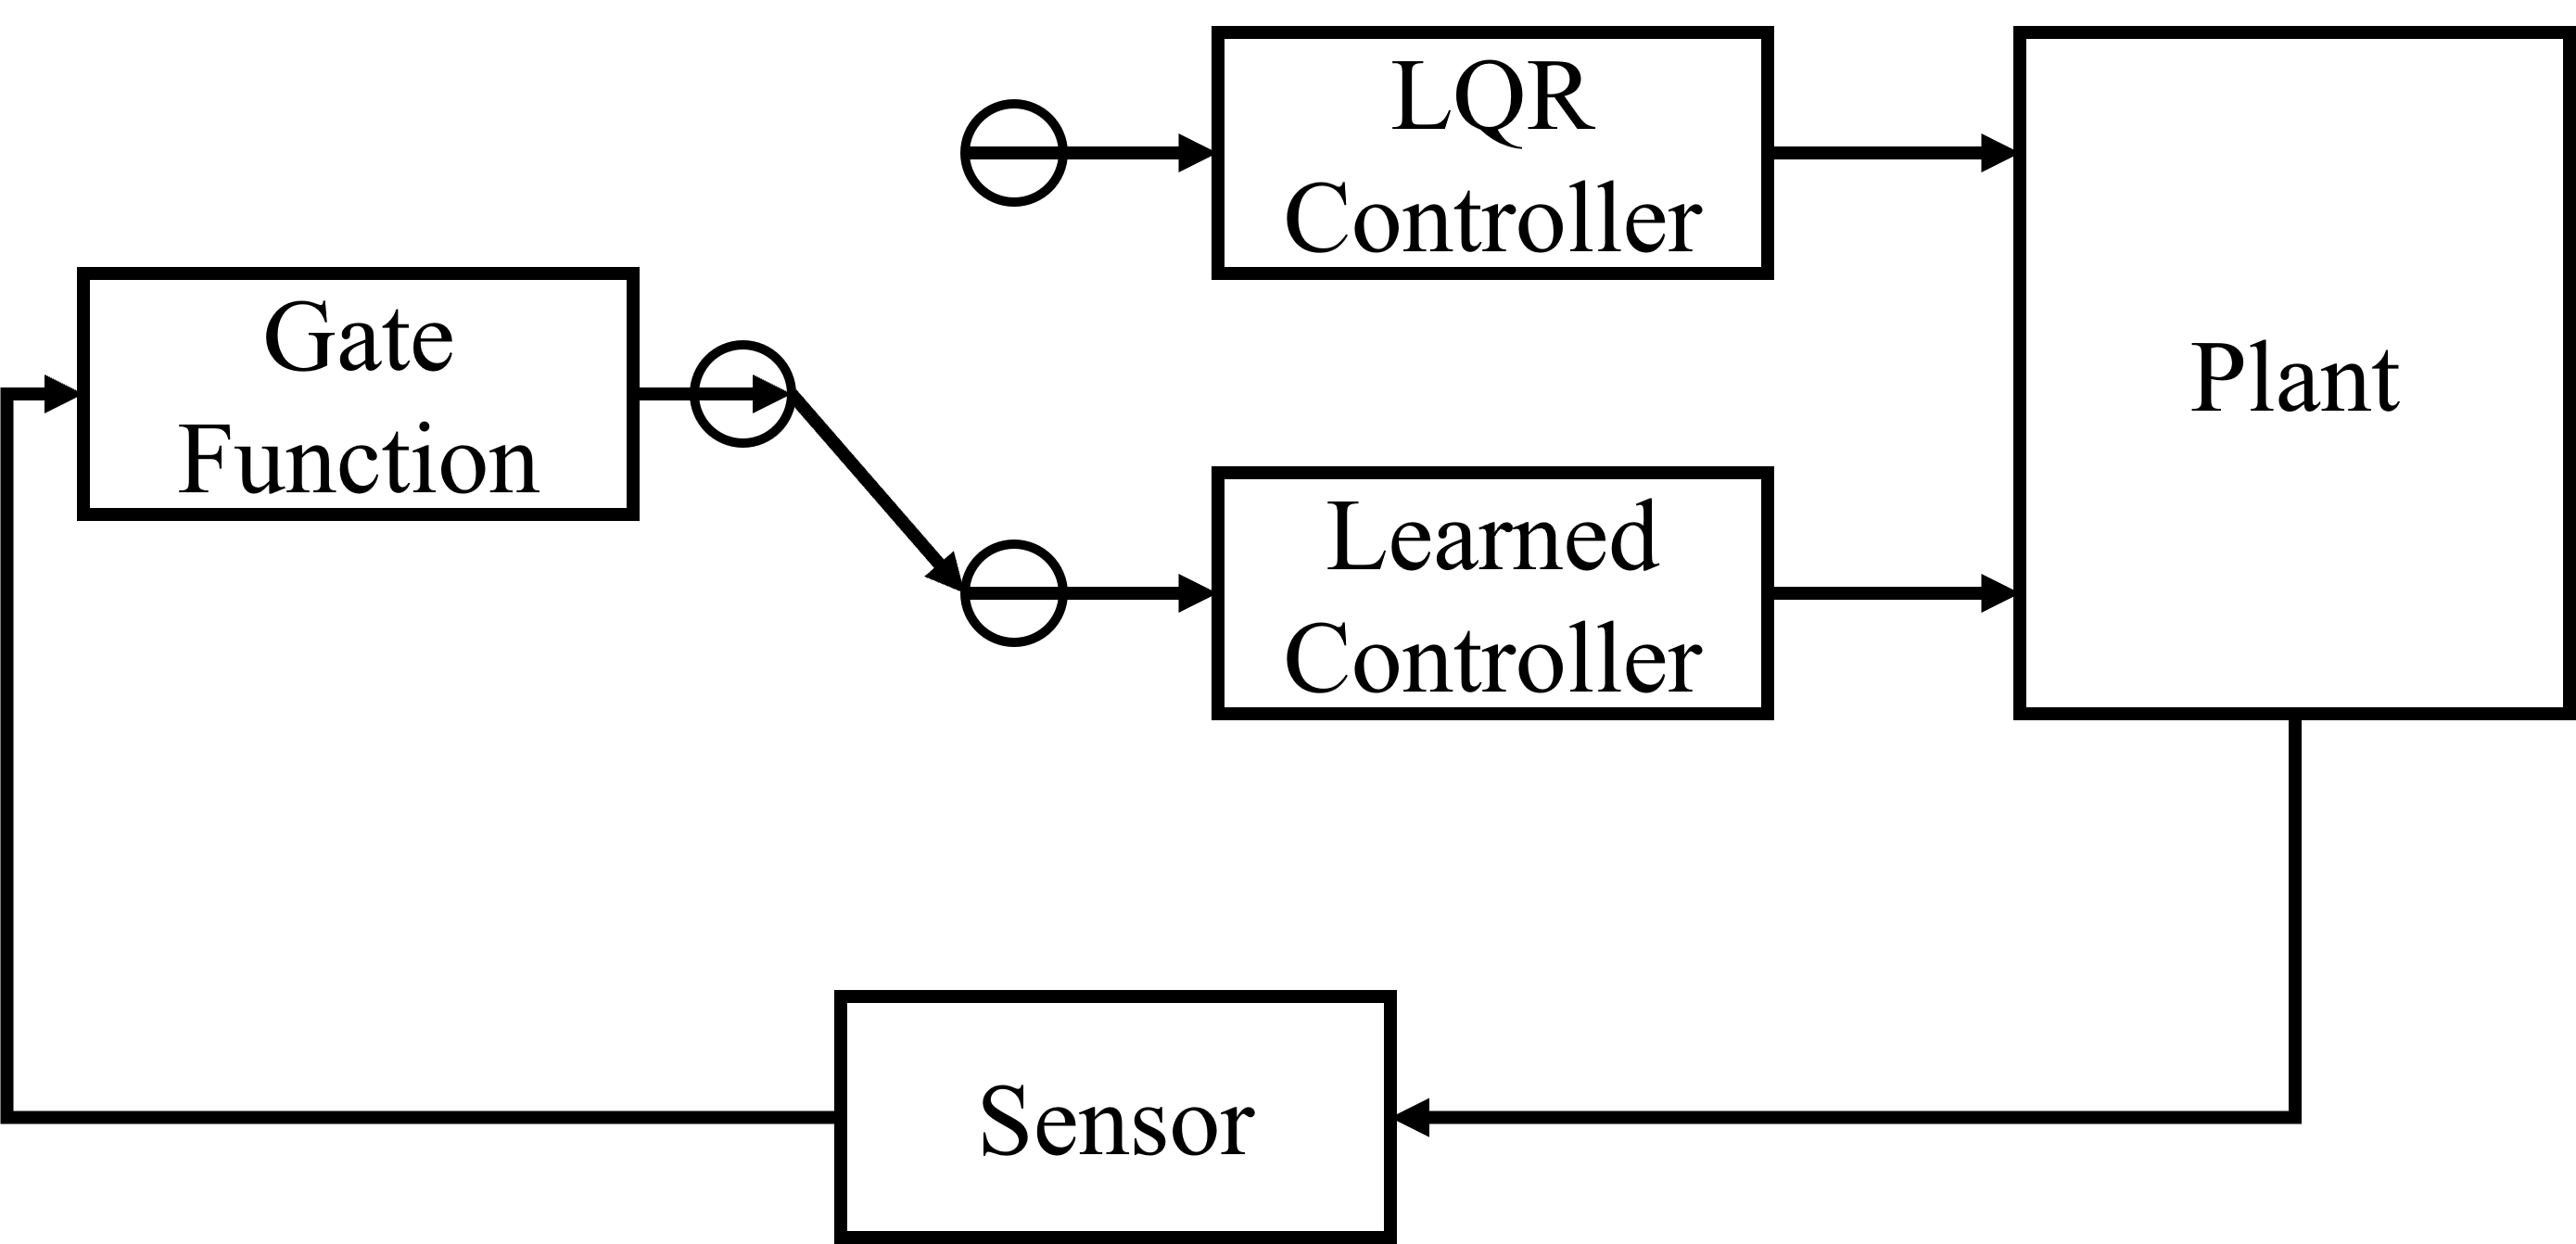
\includegraphics[width=0.8\textwidth]{figures/methodology/combined_controller.png}
    \caption{Combined controller}
    \label{fig:combined_controller}
\end{figure}

The region of attraction (RoA) for a nonlinear system, denoted as \(R_a\), describes the set of initial states surrounding a fixed point \(x_0\). If a state lies within this region, the system will converge towards \(x_0\) as \(t \rightarrow \infty\). In the context of an LQR controller, the RoA signifies the area within the state space where the controlled system exhibits asymptotic stability. For complex systems, directly computing \(R_a\) can be challenging; instead, it is often estimated. The simplest way to estimate such a set requires the assistance of a Lyapunov function \(V(x)\) bounded by a scalar \(\rho\)\cite{khalil2002nonlinear}.

\begin{equation}
 B = \{x|V(x)<\rho\}
\end{equation}

Here, \(B\) represents the estimated subset of the real region of attraction \(R_a\). 

The goal is to find the largest \(\rho\) for which the Lyapunov conditions are satisfied. These conditions are as follows:

\begin{equation}
\begin{cases}
   V(x) > 0 \\
   \dot{V}(x) < 0 & \text{for} \quad x \in B
\end{cases}
\label{eq:V_conditions}
\end{equation}

The Lyapunov function for a controlled linear system, \(\dot{x}(t) = (A - BK)x(t)\), is chosen in a quadratic form:

\begin{equation}
  V(x) = x^T S_{LQR} x 
  \label{eq:V}
\end{equation}

Here \(S_{LQR}\) is a positive definite matrix. This function serves as an 'energy-like' metric. Next, we calculate the time derivative of the Lyapunov function.For the infinite horizon LQR, \(\frac{\partial S_{LQR}}{\partial t} = 0\) and \(\frac{\partial x_0}{\partial t} = 0\), hence, \(\dot{V}\) is:

\begin{equation}
\dot{V}(x) = 2x^{T}S_{LQR}\dot{x}
\label{eq:V_dot}
\end{equation}

Combining equations and conditions \ref{eq:V_conditions}, \ref{eq:V}, \ref{eq:V_dot}, we have the following expression:

\begin{equation}
\begin{cases}
    B = \{ x \mid 0 < V(x) < \rho \} \\
    \dot{V}(x) = 2x^T S_{LQR} \dot{x} < 0
\end{cases}
\end{equation}

The RoA is computed similar to \cite{maywald2022co} but with a sums of squares method\cite{tedrake2010lqr}. The resulting shape of the RoA in a 4D state space resembles an ellipsoid.

% \begin{figure}[H]
%     \centering
%     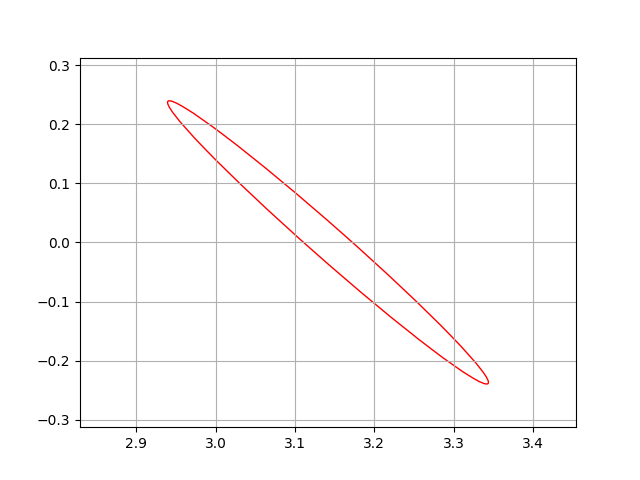
\includegraphics[width=0.6\textwidth]{figures/methodology/roaplot.png} % Adjust the width as needed
%     \caption{Region of Attraction[redraw this figure]}
%     \label{fig:example}
% \end{figure}

Once the RoA is computed, it can be checked whether a state \(x\) belongs to the estimated RoA of the LQR controller by calculating the cost-to-go of the LQR controller with the matrix \(S_{LQR}\) and comparing it with the scalar \(\rho\).

\section{Reward shaping}
The reward function is intended to guide the agent in performing desired behavior. In our design, the reward function aims to guide the double pendulum system towards achieving stability around the highest point.

One of the primary reasons why controlling an underactuated double pendulum system using RL is so challenging is the state space that can lead to successful stabilization is very small. Initial training attempts using OpenAI Gym Acrobot-v1\cite{towers_gymnasium_2023} rewards have revealed this challenge. For instance, the agent may accidentally get close to the goal state but not receive enough reward. This can result in being stuck in an unsuitable position for an extended period or a high-speed rotation of the second link with the first link almost upright. 

Another significant challenge in our RL-based training is that, due to our plan for real hardware deployment, the dynamic model of the double pendulum is more detailed than that of most simulation environments like OpenAI Gym Acrobot-v1\cite{towers_gymnasium_2023}. Because we are using quasi-direct drive motors to simplify joint dynamics, one of the significant drawbacks of this motor type is its low gear ratio, resulting in a relatively low torque limit (5 Nm).

Therefore, there is a need for an innovative reward function design suitable for our problem setup. To tackle the swing-up issue, a customized three-stage reward function is designed to steer the agent away from problematic local minima and into the region of attraction of the LQR controller. The full equation for this reward function is:

\begin{equation}
\begin{aligned}
 r(x,u) = &-(x - x_g)^T Q_{train} (x - x_g) - u^T R_{train}u \\
           & +
            \begin{dcases*}
              r_{line} & \text{if} $h(p_1, p_2) \geq h_{line}$\, ,\\
              0 & \text{else}
            \end{dcases*}\\
           & +
            \begin{dcases*}
              r_{LQR} & \text{if} $(x - x_g)^T S_{LQR} (x - x_g) \geq \rho $\, ,\\
              0 & \text{else}
            \end{dcases*}\\
           & -
            \begin{dcases*}
              r_{vel} & \text{if} $|v_1| \geq v_{thresh}$\, ,\\
              0 & \text{else}
            \end{dcases*}\\
           & -
            \begin{dcases*}
              r_{vel} & \text{if} $|v_2| \geq v_{thresh}$\, ,\\
              0 & \text{else}
            \end{dcases*}
\end{aligned}
\end{equation}

In the initial stage, a quadratic reward function is employed to encourage
smooth swinging of the entire system within a relatively small number of
training sessions. The matrix  \(Q_{train} = diag(Q_1, Q_2, Q_3, Q_4)\) is a
diagonal matrix, while \(R_{train}\) is a scalar. This is due to the nature
of underactuated control in the double pendulum system, where only a single
control input is available.

\begin{figure}[H]
    \centering
    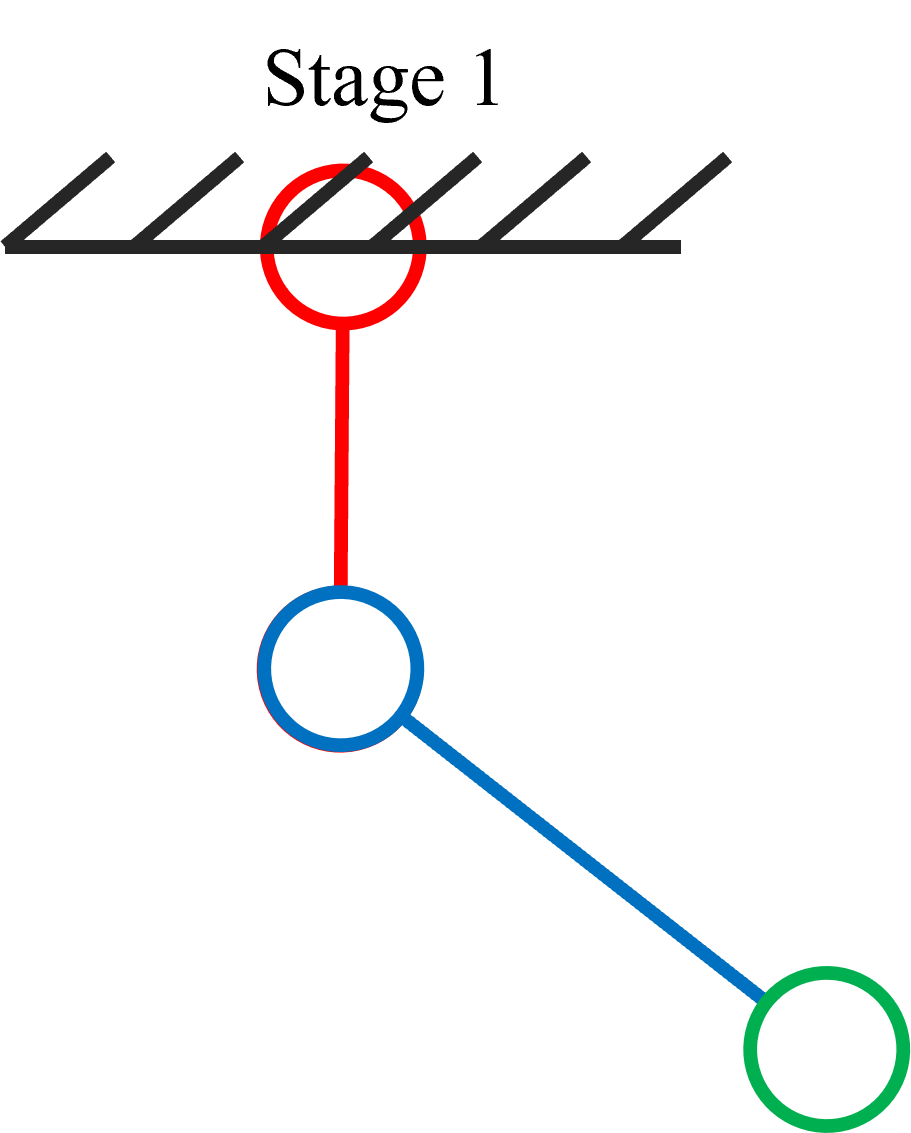
\includegraphics[width=0.25\textwidth]{figures/methodology/stage1.png} % Adjust the width as desired
    \caption{Swing up stage 1}
    \label{fig:stage1} % Optional label for referencing
\end{figure}

As the end effector reaches a threshold line \(h_{line} = 0.8(l_1+l_2)\), we
introduce a second level of reward \(r_{line}\). The end effector height is
given by
\begin{align}
    h(p_1, p_2) = -l_1\cos(p_1) - l_2 \cos(p_1 + p_2).
\end{align}

with the link lengths $l_1$ and $l_2$.
This reward provides the agent with a fixed value
but is carefully designed to prevent the system from spinning rapidly in either
clockwise or counterclockwise directions. To discourage the agent from
exploiting rewards by spinning at excessive speeds, a significant penalty
\(-r_{vel}\) is implemented for any speed exceeding $v_{thresh}=8\,
\text{rad}/\text{s}$ in absolute value.
This penalty effectively compels the agent to approach the maximum point while
adhering to the predefined speed interval(less than 20 rad/s). The speed penalty was only needed for the acrobot when the experiments are confined in simulation.

\begin{figure}[H]
    \centering
    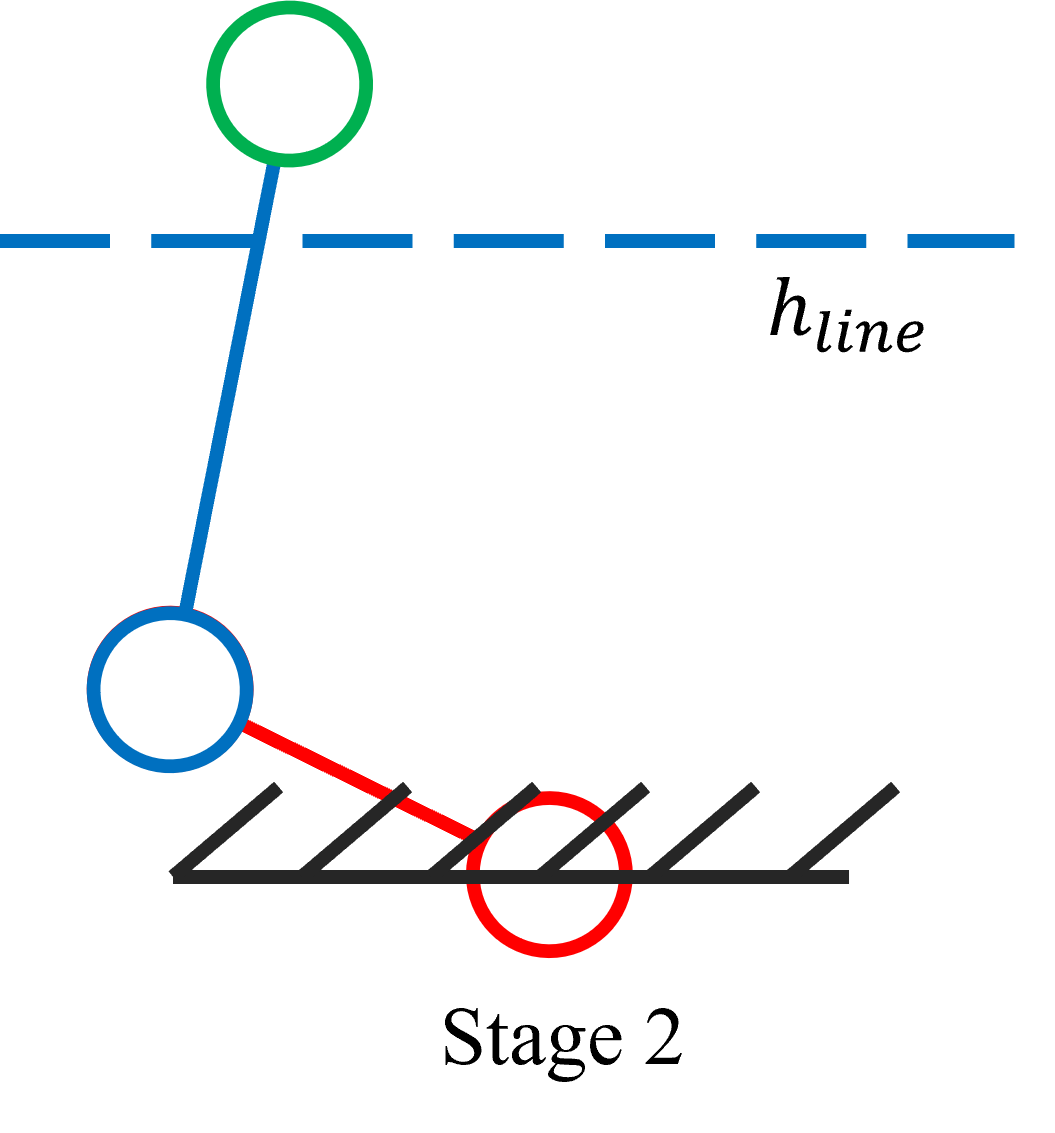
\includegraphics[width=0.25\textwidth]{figures/methodology/stage2.png} % Adjust the width as desired
    \caption{Swing up stage 2}
    \label{fig:stage2} % Optional label for referencing
\end{figure}

The third level of reward $r_{LQR}$ aims to provide a substantial reward to the
agent when it remains within the Region of Attraction (RoA) of the LQR
controller. By this we want to achieve that the policy learns to enter the LQR
controller RoA so that there can be a smooth transition between both
controllers.  The parameters, we used in
the cost matrices of the LQR controller are listed in
Table~\ref{tab:training_parameters}. 

\begin{figure}[H]
    \centering
    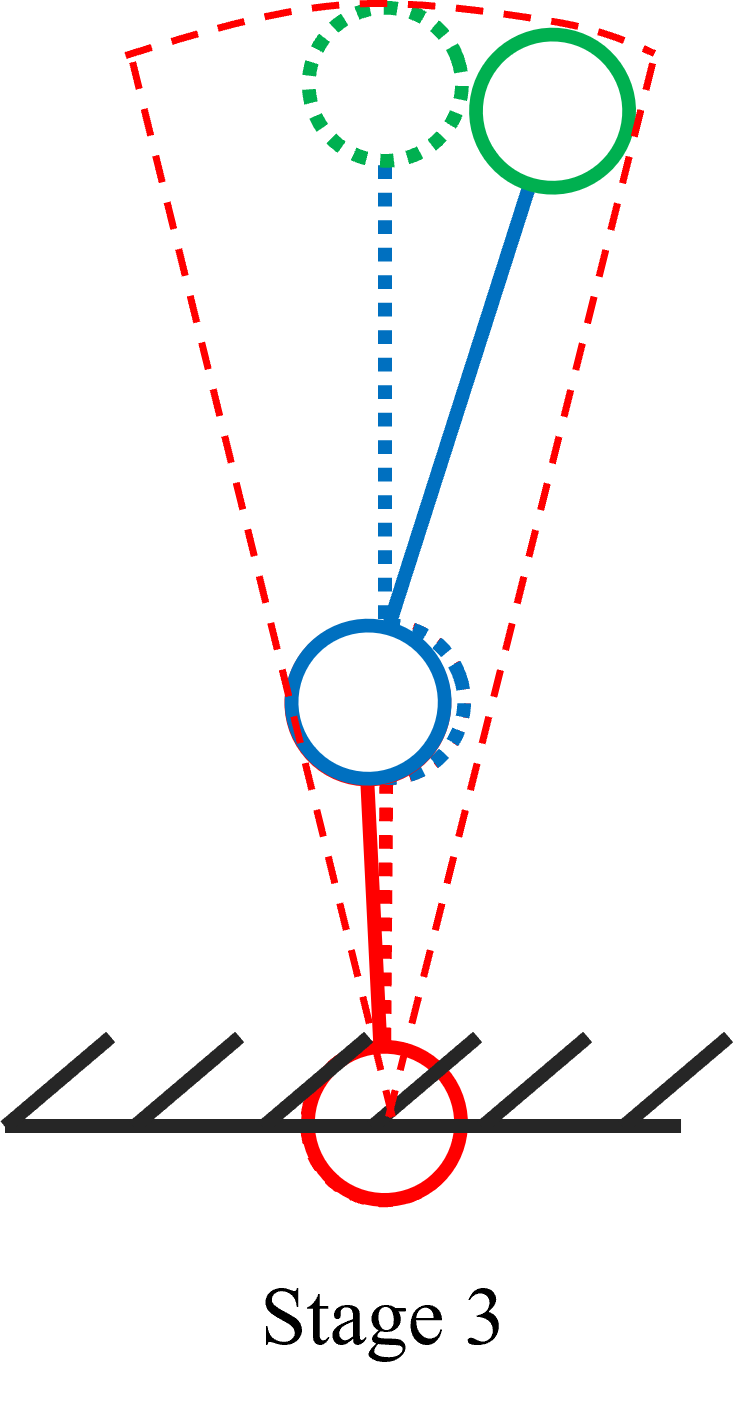
\includegraphics[width=0.2\textwidth]{figures/methodology/stage3.png} % Adjust the width as desired
    \caption{Swing up stage 3}
    \label{fig:stage3} % Optional label for referencing
\end{figure}


\section{Introduction to leaderboard metrics}
To facilitate a comparison of controller performance for the double pendulum testbench, three separate leaderboards have been created: the simulation leaderboard, the robustness leaderboard, and the real system leaderboard\cite{2023_ram_wiebe_double_pendulum}. Each of these leaderboards is additionally divided into two categories, which are determined by the pendubot and acrobot configurations.

\subsection{Performance Leaderboard in Simulation and Real system}
In the evaluation of controller performance, a set of metrics is utilized that extends beyond mere task success, delving into the finer aspects of controller operation. The same performance evaluation metrics are consistently applied to experiments conducted in both simulation environments and on real hardware. These metrics encompass various aspects, ranging from fundamental swing-up maneuver success to detailed examinations of energy consumption and torque utilization. Below, we provide a comprehensive breakdown of each metric:

\begin{itemize}
  \item \textbf{Swingup Success} \(c_{\text{success}}\):
  Determines if the end-effector successfully remains above the predefined threshold by the simulation's conclusion.
  
  \item \textbf{Swingup Time} \(c_{\text{time}}\):
  Measures the duration taken for the pendubot or acrobot to achieve and maintain its position above the threshold line. The metric only considers the swingup successful if the end-effector remains above the threshold until the simulation's end.
  
  \item \textbf{Energy} \(c_{\text{energy}}\):
  Quantifies the total mechanical energy expended during the task.
  
  \item \textbf{Max Torque} \(c_{\tau, \text{max}}\):
  Captures the highest torque applied at any point during the task.
  
  \item \textbf{Integrated Torque} \(c_{\tau, \text{integ}}\):
  Represents the cumulative torque applied throughout the task's duration.
  
  \item \textbf{Torque Cost} \(c_{\tau, \text{cost}}\):
  A quadratic metric that weighs the torques used, defined as \(c_{\tau, \text{cost}} = \sum u^TRu\), where \(R = 1\).
  
  \item \textbf{Torque Smoothness} \(c_{\tau, \text{smooth}}\):
  Reflects the variability or fluctuations in the torque signals by measuring their standard deviation.
  
  \item \textbf{Velocity Cost} \(c_{\text{vel, cost}}\):
  A metric assessing the joint velocities achieved, computed as \(c_{\text{vel}} = \dot{q}^T Q \dot{q}\), with \(Q\) being the identity matrix.
\end{itemize}

The cumulative RealAI Score is determined based on the specified formula, using the following criteria:

\begin{equation}
\begin{aligned}
S = c_{\text{success}} \Bigg(& w_{\text{time}}\frac{c_{\text{time}}}{n_{\text{time}}} + \\
& w_{\text{energy}}\frac{c_{\text{energy}}}{n_{\text{energy}}} +
w_{\tau, \text{max}}\frac{c_{\tau, \text{max}}}{n_{\tau, \text{max}}} +
w_{\tau, \text{integ}}\frac{c_{\tau, \text{integ}}}{n_{\tau, \text{integ}}} + \\
& w_{\tau, \text{cost}}\frac{c_{\tau, \text{cost}}}{n_{\tau, \text{cost}}} +
w_{\tau, \text{smooth}}\frac{c_{\tau, \text{smooth}}}{n_{\tau, \text{smooth}}} +
w_{\text{vel, cost}}\frac{c_{\text{vel, cost}}}{n_{\text{vel, cost}}} \Bigg)
\end{aligned}
\end{equation}

The weights and normalizations are:
\begin{table}[H]
  \centering
  \begin{tabular}{lcc}
    \hline
    Criteria & Normalization \(\mathit{n}\) & Weight \(\mathit{w}\) \\
    \hline
    Swingup time & 10.0 & 0.2 \\
    Energy & 100.0 & 0.1 \\
    Max. Torque & 6.0 & 0.1 \\
    Integrated Torque & 60.0 & 0.1 \\
    Torque Cost & 360 & 0.1 \\
    Torque Smoothness & 12.0 & 0.2 \\
    Velocity Cost & 1000.0 & 0.2 \\
    \hline
  \end{tabular}
  \caption{Weights and normalizations for performance leaderboards}
  \label{tab:performance}
\end{table}

In the simulation experiments, the pendubot is modeled using a Runge-Kutta 4 integrator with a timestep of \(dt=0.002s\) over a span of \(T=10s\). The pendubot is initiated in a hanging down configuration, represented as \(x_0 = [0, 0, 0, 0]^T\), with the goal of reaching the unstable fixed point in the upright configuration, denoted as \(x_g = [\pi, 0, 0, 0]^T\). The double pendulum is considered to have achieved its upright position once the end-effector surpasses the threshold line situated at \(h=0.45m\), with the origin being the mounting point.

In real hardware experiments, there exists a torque limit of 0.5 Nm on the passive joint, which compensates for the motor's friction. The actuators are capable of operating at a control frequency as high as 500Hz, and each experiment has a duration of 10 seconds. The pendubot commences from a hanging down position, aiming to reach the unstable fixed point in the upright configuration. Successful attainment of the upright position is confirmed when the end-effector crosses the threshold line set at \(h=0.45m\), measured from the mounting point's origin.

\subsection{Simulation Robustness Leaderboard}
In addition to performance metrics, we also consider robustness metrics. As the ultimate goal is to transfer successful models from a simulation environment to real hardware, it's essential to assess the robustness of controllers developed within the simulation. This helps determine the types of perturbations that affect each controller.

\begin{itemize}
    \item \textbf{Model Inaccuracies \(c_{model}\)}: Model parameters determined through system identification are inherently subject to inaccuracies. To assess these inaccuracies, variations are introduced one at a time into the independent model parameters within the simulator while maintaining the use of the original model parameters in the controller.

    \item \textbf{Velocity Measurement Noise \(c_{vel, noise}\)}: The outputs of the controllers depend on the measured system state, and in the case of the QDDs, online velocity measurements introduce noise. Therefore, it is important for transferability that a controller can handle at least this level of noise in the measured data. Testing is conducted with and without a low-pass noise filter.
    
    \item \textbf{Torque Noise \(c_{\tau,noise}\)}: Beyond measurement noise, the torque output by the controller may not precisely match the desired value.

    \item \textbf{Torque Response \(c_{\tau,response}\)}: The controller's requested torque typically varies during execution, and the motor may not be able to instantaneously respond to significant torque changes. Instead, it may overshoot or undershoot the desired torque value. This behavior is modeled by the equation \(\tau = \tau_{t-1} + k_{\text{resp}} (\tau_{\text{des}} - \tau_{t-1})\), where \(\tau_{\text{des}}\) is the desired torque. In this model, a \(k_{\text{resp}}\) value of 1 indicates flawless torque response, while any deviation from 1 indicates imperfect motor responses.

    \item \textbf{Time Delay \(c_{delay}\)}: In real-system operations, time delays inevitably arise due to communication and reaction times. It's essential to account for these when evaluating controller performance.
\end{itemize}

The above criteria are employed to compute the comprehensive RealAI Score using the given formula:
\begin{equation}
 S = w_{model} c_{model} + 
    w_{vel, noise} c_{vel, noise} +  
    w_{\tau, noise} c_{\tau, noise} +  
    w_{\tau, response} c_{\tau, response} +  
    w_{delay} c_{delay}
\end{equation}

The weights are:
\begin{equation}
 w_{model} = w_{vel, noise} = w_{\tau, noise} = w_{\tau, response} = w_{delay} = 0.2
\end{equation}
\cleardoublepage
